\documentclass{beamer}
%
% Choose how your presentation looks.
%
% For more themes, color themes and font themes, see:
% http://deic.uab.es/~iblanes/beamer_gallery/index_by_theme.html
%
\mode<presentation>
{
  \usetheme{default}      % or try Darmstadt, Madrid, Warsaw, ...
  \usecolortheme{default} % or try albatross, beaver, crane, ...
  \usefonttheme{default}  % or try serif, structurebold, ...
  \setbeamertemplate{navigation symbols}{}
  \setbeamertemplate{caption}[numbered]
} 

\usepackage[english]{babel}
\usepackage[utf8x]{inputenc}
\usepackage{graphicx}
\usepackage{listings}

\graphicspath{{img/}}

\title[State Space Search Algorithms]{State Space Search Algorithms}
\author{Vedran Pintarić}
\date{15.11.2018.}

\begin{document}

\begin{frame}
  \titlepage
\end{frame}

\section{Problem definition}

\begin{frame}{Problem definition}

\begin{itemize}
	\item a set of states (state space)
	\item initial state
	\item transitions between states
	\item goal state test
\end{itemize}

\end{frame}

\begin{frame}[fragile]{Problem definition}

\begin{lstlisting}[language=Python]
class Problem:
	# Should return a State object
	def getInitialState(self):
		pass

	# Should check if given
	# state is goal state
	def isGoalState(self, state):
		pass

	# Should return a list
	# of triplets (state, action, cost)
	def getSuccessors(self, state):
		pass
\end{lstlisting}

\end{frame}

\subsection{8-Puzzle}

\begin{frame}
\begin{figure}
\centering
	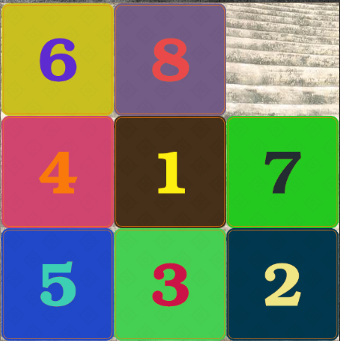
\includegraphics[width=0.5\linewidth]{puzzle8.png}
	\caption{8-Puzzle initial state}
\end{figure}
\end{frame}

\begin{frame}
\begin{figure}
\centering
	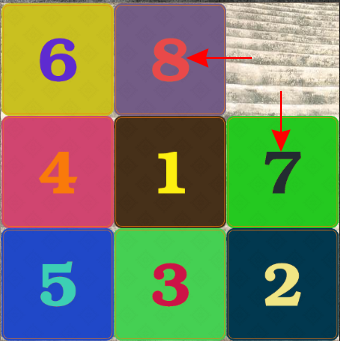
\includegraphics[width=0.5\linewidth]{puzzle8_arrows.png}
	\caption{8-Puzzle possible actions}
\end{figure}
\end{frame}

\begin{frame}
\begin{figure}
\centering
	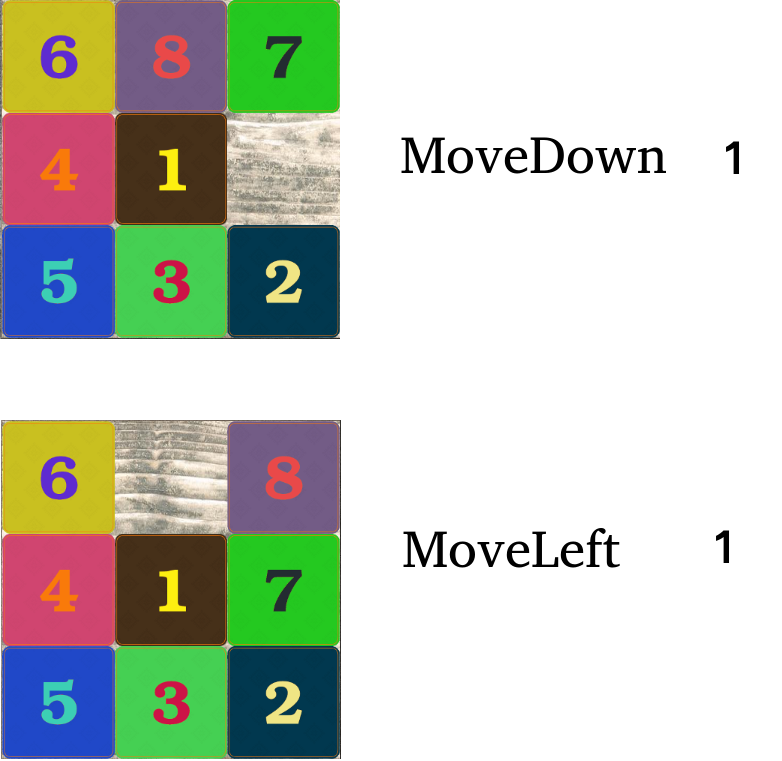
\includegraphics[width=0.5\linewidth]{puzzle8_successors.png}
	\caption{8-Puzzle list of successor triplets}
\end{figure}
\end{frame}

\begin{frame}
\begin{figure}
\centering
	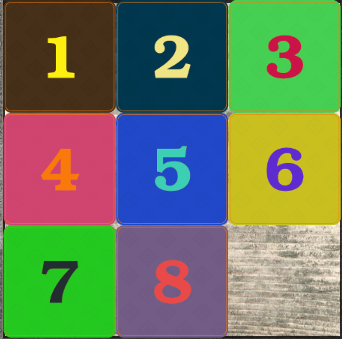
\includegraphics[width=0.5\linewidth]{puzzle8_goal.png}
	\caption{8-Puzzle goal state}
\end{figure}
\end{frame}

\subsection{Pathfinding}

\begin{frame}
\begin{figure}
\centering
	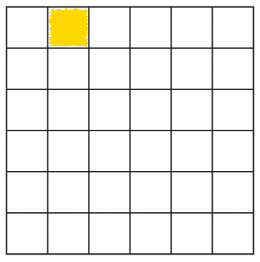
\includegraphics[width=0.5\linewidth]{pathfinding.png}
	\caption{Pathfinding initial state}
\end{figure}
\end{frame}

\begin{frame}
\begin{figure}
\centering
	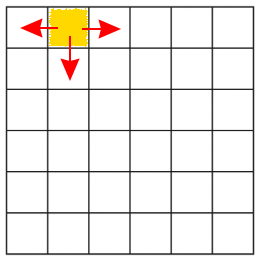
\includegraphics[width=0.5\linewidth]{pathfinding_arrows.png}
	\caption{Pathfinding possible actions}
\end{figure}
\end{frame}

\begin{frame}
\begin{figure}
\centering
	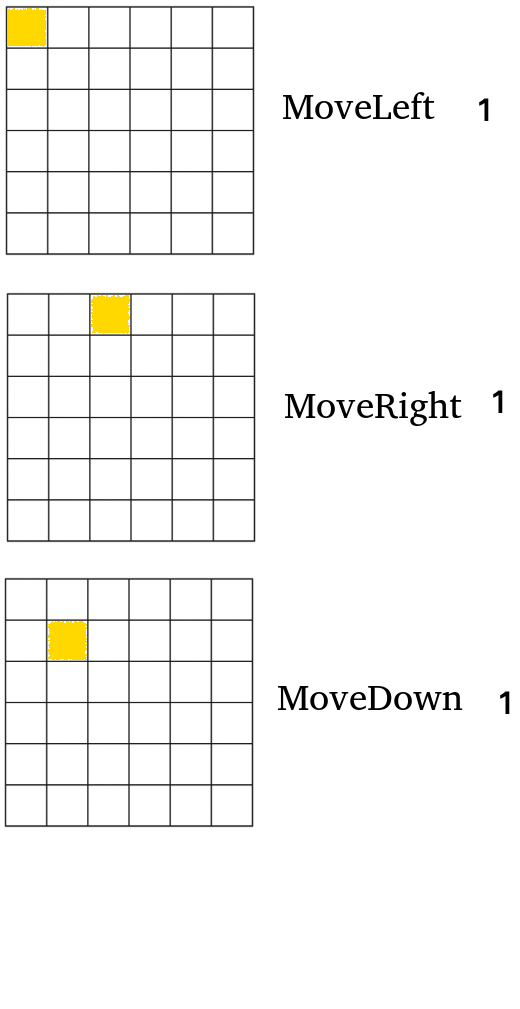
\includegraphics[width=0.3\linewidth]{pathfinding_successors.png}
	\caption{Pathfinding list of successor triplets}
\end{figure}
\end{frame}

\begin{frame}{State space graph}
\pause
\begin{figure}
\centering
	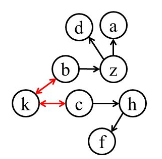
\includegraphics[width=0.6\linewidth]{state_space_graph.png}
	\caption{State space graph}
\end{figure}
\end{frame}

\section{Search algorithm}

\subsection{Search tree}

\begin{frame}{Search tree}

\begin{figure}
\centering
	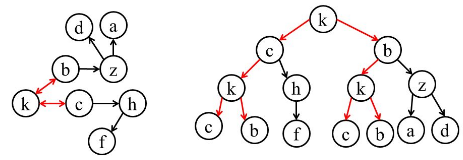
\includegraphics[width=\linewidth]{state_space_vs_search_tree.png}
	\caption{State space vs search tree}
\end{figure}

\end{frame}

\begin{frame}{Nodes}

\begin{itemize}
	\item Open nodes - known but unexplored
	\item Closed nodes - explored i.e. checked against goal state and their successors were queried
\end{itemize}

\end{frame}

\subsection{General algorithm pseudocode}

\begin{frame}[fragile]{General algorithm pseudocode}
\begin{lstlisting}
openNodes.insert(getInitialState())
while openNodes not empty 
	node = openNodes.get()
	if isGoalState(node)
		return node
	for childNode in getSuccessors(node)
		openNodes.insert(childNode)
\end{lstlisting}
\end{frame}

\section{Blind algorithms}

\subsection{Breadth first search (BFS)}

\subsection{Depth first search (DFS)}

\subsection{Uniform cost search}


\section{Heuristic algorithms}

\subsection{Heuristics}

\subsection{Greedy search}

\subsection{A* search}


\section{Unity engine - NavMesh}


% -----------------------------------------

\section{Introduction}

\begin{frame}{Introduction}

\begin{itemize}
  \item Your introduction goes here!
  \item Use \texttt{itemize} to organize your main points.
\end{itemize}

\begin{block}{Examples}
Some examples of commonly used commands and features are included, to help you get started.
\end{block}

\end{frame}

\section{Some \LaTeX{} Examples}

\subsection{Tables and Figures}

\begin{frame}{Tables and Figures}

\begin{itemize}
\item Use \texttt{tabular} for basic tables --- see Table~\ref{tab:widgets}, for example.
\item You can upload a figure (JPEG, PNG or PDF) using the files menu. 
\item To include it in your document, use the \texttt{includegraphics} command (see the comment below in the source code).
\end{itemize}

% Commands to include a figure:
%\begin{figure}
%\includegraphics[width=\textwidth]{your-figure's-file-name}
%\caption{\label{fig:your-figure}Caption goes here.}
%\end{figure}

\begin{table}
\centering
\begin{tabular}{l|r}
Item & Quantity \\\hline
Widgets & 42 \\
Gadgets & 13
\end{tabular}
\caption{\label{tab:widgets}An example table.}
\end{table}

\end{frame}

\subsection{Mathematics}

\begin{frame}{Readable Mathematics}

Let $X_1, X_2, \ldots, X_n$ be a sequence of independent and identically distributed random variables with $\text{E}[X_i] = \mu$ and $\text{Var}[X_i] = \sigma^2 < \infty$, and let
$$S_n = \frac{X_1 + X_2 + \cdots + X_n}{n}
      = \frac{1}{n}\sum_{i}^{n} X_i$$
denote their mean. Then as $n$ approaches infinity, the random variables $\sqrt{n}(S_n - \mu)$ converge in distribution to a normal $\mathcal{N}(0, \sigma^2)$.

\end{frame}

\end{document}